%!TEX root = ../thesis.tex

\section{EX.1}
ロータリージョイントを持つ単リンクロボットは, 初期位置であるθ = 15度で静止している. このロボットを滑らかに動かし, 3秒で目標位置であるθ = 75度に移動させたい. この動作を実現し, マニピュータを目標位置で停止させるための3次関数の係数を求める. そして, 時間の関数としてジョイントの位置, 速度, および加速度をプロットする. \\

式(6)に代入すると, 次のようになる.

$$a_0 = 15.0$$
$$a_1 = 0.0$$
$$a_2 = 20.0 \eqno(7)$$
$$a_3 = -4.44$$

式(3)と(4)を用いて, 次のように得られる.

$$θ(t) = 15.0 + 20.0t^2 -4.44t^3$$
$$\dot{θ}(t) = 40.0t - 13.33t^2 \eqno(8)$$
$$\ddot{θ}(t) = 40.0 -26.66t$$

\figref{Fig:fig2}は, この動作を40 Hzでサンプリングした際の位置, 速度, および加速度関数を示している. 任意の3次関数の速度プロファイルが放物線であり, 加速度プロファイルが直線であることに注意したい. 

\begin{figure}[h]
  \centering
  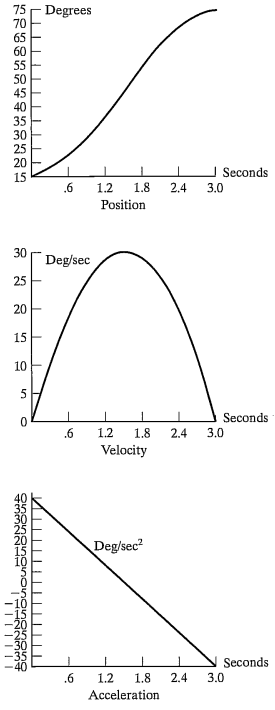
\includegraphics[keepaspectratio, scale=0.6]{images/fig2.png}
  \caption{}
  \label{Fig:fig2}
  \end{figure}